The crowdsourcing media annotation method presented in this paper follows three steps: Preparation, Annotation, and Presentation. In the preparation step, the production process is defined, in the annotation step the contributions are collected and processed and, in the presentation step, the outcome is available for consumption.

\subsection{Preparation} 
All activities involved in this step are performed by the owner, who started the media annotation process. The complex media annotation desired as a result is analyzed and all information required for its construction is identified.

Then it is necessary to determine the simple annotation tasks required to obtain this information and the order of dependency between the tasks. For each of these tasks, it is necessary to define:
\begin{itemize}
\item What kinds of point of interest should be annotated.\\Ex: events, objects, subjects, issues.
\item What annotation type will be used for each of these kinds.\\Ex: free write, item selection, button click, image upload.
\item What data type will be collected for each annotation type.\\Ex: plain text, location, image, video.
\end{itemize}

%To illustrate this point, the example of the football(soccer) match annotation will be recalled. In a football(soccer) match video the kinds of point of interest correspond to events such as goals, cards, and faults. For each point of interest observed it should be collected its kind, and the instant when this event happened. The annotation type to be used on the annotation tool can be a set of icons related to each event. Finally, the data type collected in this case may be plain text that contains the kind of event identified and the instant it happened \cite{santos2007estrategia}.

Once the simple media annotation microtasks are defined, a workflow can be constructed to determine how they fit into the complex annotation production process. The built workflow should follow the general model shown in Figure ~\ref{method}. This workflow will guide the annotation step.

\begin{figure}[h]
	\centerline{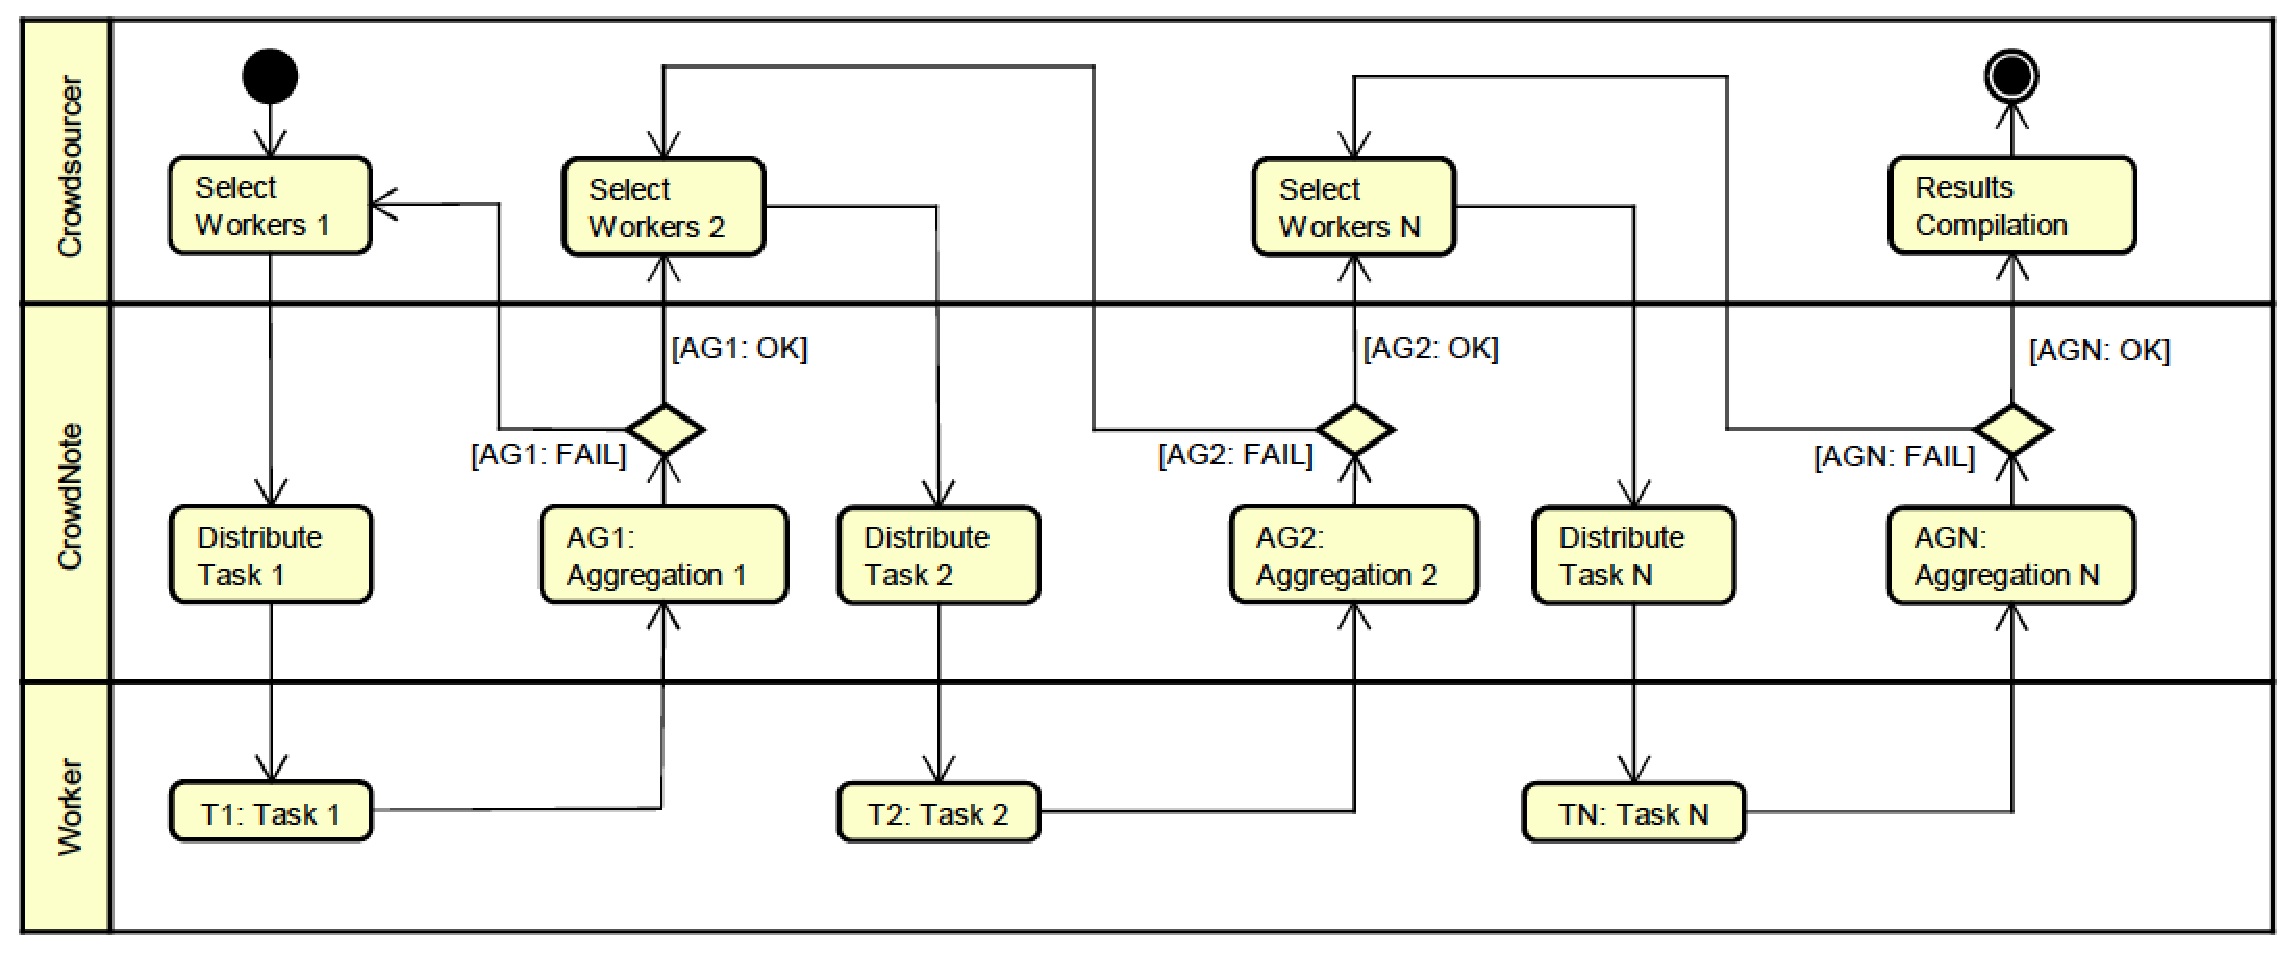
\includegraphics[scale=0.22] {figure/method}}
	\caption{Process workflow}
	\label{method}
\end{figure}


Also, it is important to provide explanations or guidelines that can instruct the workers about how to execute the microtasks. An additional activity on the Preparation step is to determine what image or segment of audio or video should be sent by each worker, this division can be made by duration (ex: send a 5 seconds segment to each worker), or using contextual criteria such as to send to each user a segment that contains a single dialog.

\subsection{Annotation}
The workflow produced in the preparation step defines how the output from a task will be used as input to the next one. In this way, the output of the last task is equal to the desired outcome of the process. In addition, each task can generate multiple outputs that are different representations of the collected and aggregated data. For example, events identified in a video by a task can either serve as input to the next task or generate indices or summaries for the video.

This cascading microtasks workflow is illustrated in Figure~\ref{method}. It is important to notice that each iteration in this workflow is composed of two activities, the task in self and the aggregation activity, that generates the output from the obtained contributions. 

The method determines that annotations are collected from the workers on each of the tasks, however, these annotations can be obtained from crowds or crowdsourcing indoor environments, or from open crowds brought together by an open call.


\subsection{Presentation} 
In the presentation step the result generated is made available, it can be displayed by a player or exported in different formats. In fact, the output can be exported in several formats, because the complex annotation generated is stored as metadata and offers flexibility in this regard.










